%%%%%%%%%%%%%%%%%%%%%%%%%%%%%%%%%%%%%%%%%%%%%%%
% CHT-20 Template / Guide For Authors. 
%%%%%%%%%%%%%%%%%%%%%%%%%%%%%%%%%%%%%%%%%%%%%%%
\documentclass[12pt]{CHT-20}
\usepackage{CHT-20}
\usepackage[utf8]{inputenc}

% SQUEO packages
\usepackage{graphicx}
%\usepackage[justification=centering]{caption}
\usepackage{subcaption}
\usepackage{float}
%\usepackage{subfig}
\usepackage{amsmath}
\usepackage{amsfonts}
\usepackage{amssymb}
\usepackage{comment}

\pnumber{CHT-21-178}
\ptitle{ SOOT PREDICTION IN FLAMES USING A DATA-BASED MACHINE LEARNING APPROACH }


\author[*,\S]{Joseph N. Squeo}
\author[*]{Xinyu Zhao}

\affil[*]{Department of Mech. Eng., University of Connecticut, Storrs, CT 06269, United States}
\affil[ \S]{Correspondence author. Email: joseph.squeo@uconn.edu}

\pabstract{Soot prediction in combustion systems remains a challenge due to the underlying complex physical processes and uncertainties in model parameters. Collecting experimental data of flames is costly with accurate measurements and often difficult to obtain for large-scale pool fires. Models of flames that provide accurate soot prediction for sufficiently accurate radiative heat transfer prediction are an efficient means to improve fire prediction and improve our understanding of fire dynamics. Following the wake of machine learning (ML) algorithms development, data from well-validated computational fluid dynamics can be used to predict soot in flames using key parameters relating to combustion. Machine learning includes data-based algorithms that involve training a model to predict an outcome.
%Many researchers use machine learning for effective model prediction, classification, and progress towards human-level AI. 
In this work, a Poisson supervised regression machine learning model is trained using several key soot-related parameters from five chemical mechanisms and tested on data from one additional chemical mechanism for an atmospheric, 1D premixed ethylene and air flame first. The methodology is extended to a well-validated dataset of a 2D atmospheric laminar diffusion flame on the Santoro burner and tested on a similar flame with modified flow conditions. The trained machine learning model is capable of predicting the location of the entire soot field with sufficiently accurate prediction of the concentration of soot.}

\begin{document}

\maketitle

\makeabstract
  
\section{Introduction}
% Motivation - CFD, thermal radiation and fires
Computational fluid dynamics (CFD) based fire models aim to capture the dynamics of fire to better understand the underlying physics~\citep[]{Roy}. Thermal radiation accounts for the majority of overall heat transfer to the ambient surroundings in large scale fires~\citep[]{DeRis1979}, and contributes to the growth and spread of fires. Therefore, the thermal radiation emitted from a fire is a fundamental quantity of interest to the fire engineering community in order to improve fire models to protect against dangerous fire spread. 

% Soot modeling
Soot is a very fine particulate substance consisting of black carbon and other impurities produced by the incomplete combustion of a hydrocarbon fuel, contributing significantly to thermal radiation in fires and combustion systems. Sufficiently accurate predictions of soot concentrations from a soot model are required for accurate predictions of thermal radiation from fires. However, significant uncertainties prevail in soot models, due to the lack of sufficient fundamental understanding of soot formation, growth and oxidation~\citep[]{Roy,modelAssessment}. Most soot models require {\em ad hoc} tuning against experimental data to adequately predict soot concentrations for specific fuels and flames. Soot has been a subject of continuing experimental and numerical studies with the goal of developing affordable and effective models to capture soot concentrations in flames. The soot and thermal radiation coupling in fires is one of the most complex phenomena involved in fire, and remains an important problem for fire engineers to better predict fires with CFD simulations.

% Machine learning overview
To circumvent the modeling difficulties imposed by soot as a means to advance the understanding of fire dynamics, a data-based machine learning technique is adopted in this study. Machine learning algorithms can learn from input training data and improve from experience without additional human intervention. Machine learning algorithms can be broadly classified into three types: supervised, unsupervised and reinforced learning~\citep[]{Vieira2019,Badillo2020}. Supervised learning, employed in this work, utilizes known input and output data to train a parametric model that can be used to predict the target output for new input data. The model learns the function that maps an input dataset to the output, and can be used for classification or regression. Unsupervised learning models determine the underlying structure of the data from input variables without any corresponding output variables. Common uses of unsupervised models include association probabilistic models, data clustering and dimensionality reduction. Lastly, reinforcement algorithms learn optimal actions through a trial and error process to maximize an objective. 

% Review of previous works
Machine learning has grown in popularity in the 21\textsuperscript{st} century with the advent of increasing computing power.
%Application of machine learning algorithms are nearly endless. 
These powerful techniques are used everyday for tasks ranging from filtering spam emails~\citep[]{Sanghani2019} to classifying regions of a combustion chamber into light and heavy sooting zones based on temperature and equivalence ratio~\citep[]{Yu2019}.
%to predicting global virus spread and infection rates~\cite{Assaf2020,Cohen2020,Zoabi2020,Zoabi2021,Ahamad2020}. 
In terms of soot prediction in combustion systems,~\citet{Alexander2018} demonstrated that an estimator library built from streamline Lagrangian histories of key parameters from CFD flame datasets could be used to predict soot concentration sufficiently well along the flame centerline.~\citet{Zimmer2019} redesigned the inexpensive soot estimator library generated from validated sooting flame models to predict the entire soot field for nine different sooting ethylene and air coflow flames.~\citet{Gao2019} predicted the sooting tendencies of oxygenated components of fuels using kernel ridge regression supervised machine learning using a training process between fuel molecular structure and sooting tendency. Predicted values of the yield sooting index were in good agreement with the measured values, allowing the method to be used to compare sooting tendencies of new fuels.~\citet{Rodriguez2019} determined the sooting propensity of an axisymmetric laminar diffusion flame using a support vector machine learning algorithm trained on images of flames captured in laboratory conditions. The classifier algorithm yielded a promising solution for non-invasive and low-cost experimental instrumentation for characterizing combustion flames by sooting propensity.
 
% Paper objective
The primary objective of this study is to demonstrate that machine learning techniques can be employed to predict soot in laboratory scale flames. A Poisson regression supervised machine learning algorithm is chosen in this work to predict soot volume fraction in target 1D and 2D atmospheric ethylene and air flames. The model is trained and tested on well-validated data generated from numerical flame simulations in \texttt{OpenFOAM}. The baseline models feature a 32-species skeletal chemical mechanism~\citep[]{Lu_skeletalMech}, a mixture-averaged molecular transport model~\citep[]{Dasgupta2015} and the two-equation soot model~\citep[]{Leung_Lindstedt_Jones} with modified oxidation reactions~\citep[]{Guo2004}. Two laminar ethylene/air diffusion flames are simulated using the baseline models and compared against available experimental measurements and the machine learning model prediction.
%The intent of this work is to extend the methodology to more complex, larger-scale flames. The regression model can be trained using scalar field solutions of simpler flames with lesser computational burden then tested on more complex target flames, such as turbulent pool fires, with sufficient accuracy.

% Paper overview
The rest of the paper is organized as follows. The Poisson regression model and numerical flame solver are discussed in Sec.~\ref{sec:methods}. The test flames and simulation details are then introduced in Sec.~\ref{sec:testFlames}. Following that, results obtained using the baseline model and machine learning procedure are compared in Sec.~\ref{sec:results}, where the predicted soot volume fraction fields are compared against the baseline solution. Conclusions are finally drawn in Sec.~\ref{sec:conclusion} with suggestion for future work.
%Lastly, Sec.~\ref{sec:acknowledgements} acknowledges the support and funding for this project.









% ======================================================= %
\section{Methods} \label{sec:methods}

\subsection{Machine learning approach}
% DISCUSS: Overview of machine learning regression approach with 1D/2D flames
A supervised Poisson regression algorithm is implemented in this work. In general, regression models seek to minimize an objective function such that the sum of squared error is minimized between the observed target parameter $y$ and the predicted value. Suppose a model $f$ can be found that maps each $P$-dimensional input parameter array $\mathbf{x}_i$ in the feature space $\mathbf{X} \in \Re^{K \times P}$ of $i=1,2,\dots,K$ samples and $P$-parameters to a value of $y'_i \in \Re^{1 \times 1}$. Function $f$ contains model parameters $\mathbf{w}$ such that
\begin{equation}
    f(\mathbf{x}_i|\mathbf{w}) = y'_i \ 
    \label{eq:modelFunction}
\end{equation}
where $\mathbf{w} \in \Re^{P \times 1}$ is an array containing the model coefficients of the linear or nonlinear model function $f$, and $y'_i$ is the i\textsuperscript{th} predicted value of the target parameter $y_i$. The general least squares object function is expressed as
\begin{equation}
    \text{min}({\mathbf{w}}): \sum^K_{i=1} \left(y_i - f(\mathbf{x}_i|\mathbf{w})\right)^2 \
    \label{eq:objectiveFunctionGeneral}
\end{equation}
Minimization of the objective function is accomplished using a gradient descent numerical technique. The regression model is trained using known discrete scalar field solutions of key parameters relating to soot from well-validated numerical simulations of 1D and 2D ethylene/air flames. Model performance is evaluated by testing the prediction of soot of the trained model on the same flame but with a unique set of data not included in the training dataset. Soot prediction is then tested on a secondary 2D ethylene/air laminar diffusion flame with different flow conditions, burner geometry and flame shape than the original flame and training dataset.

% DISCUSS: Poisson regression - what is it and formulation (penalty coefficients)
Poisson regression is a count-based regression model that interprets the training dataset as the number of times a particular soot volume fraction occurs at a corresponding combination of the feature space parameters. An operator maps the training samples of $P$-dimensions to $P$-regression coefficients, $\mathbf{w}$. Poisson regression uses a natural exponent term to represent the model function operator $f$ such that 
\begin{equation}
    f(\mathbf{X}|\mathbf{w}) = \exp{(\mathbf{X}\mathbf{w})} = \mathbf{y}' \
\end{equation}
where $\mathbf{X}$ is feature space matrix comprised of the $P$-dimensional training parameters $x_i$ for $i=1,2,\dots,K$ samples. The objective function that Poisson regression seeks to minimize contains a penalty term that penalizes the model parameter coefficients $\mathbf{w}$ to reduce the risk of over and under fitting of the model. The objective function is expressed as
\begin{equation}
    \text{min}({\mathbf{w}}): \sum^K_{i=1} \left(y_i - \exp{(\mathbf{x_i}\mathbf{w})}\right)^2 + \alpha||\mathbf{w}||_2 \ 
    \label{eq:objectiveFunctionPoisson}
\end{equation}
where $\alpha$ is the scalar penalty coefficient bounded between zero and unity and $||\mathbf{w}||_2$ represents the Euclidean L\textsubscript{2}-norm
\begin{equation}
    ||\mathbf{\gamma}||_2 = \sum_i \gamma_i^2 \ 
\end{equation}
Compared to several regularized regression techniques tested including Lasso and Ridge regression, Poisson regression yielded much better predictions of soot volume fraction in the tested flames and avoids the complications of negative, nonphysical predictions that other regression models naturally face when the training data is small and near zero.

% DISCUSS: regression procedure in Python (nonlinear mappings,normalizing, ln transform, sciPy,...)
The Poisson regression model used in this work is implemented in \texttt{Python} using the \texttt{Scikit learn}~\citep[]{scikit-learn} machine learning package. Scalar fields of key parameters related to the soot formation processes from well-validated numerical flame simulations of 1D and 2D ethylene/air flames are mapped to a higher order, nonlinear feature space consisting of all linear combinations of the parameters up to the specified polynomial degree. Once the features are mapped, the natural logarithm of each feature is computed, transforming the feature space into an exponential space to prevent negative, nonphysical predictions of soot. Before the regression model is trained using the feature space, the features are normalized such that each feature is rescaled between zero and unity to remove the mixture of scales present between the combustion related parameters $X$, where the normalized feature parameter $X'$ is expressed as
\begin{equation}
    X' = \frac{X-X_{min}}{X_{max}-X_{min}} \ 
\end{equation}
Pre-processing the feature space is crucial for the effectiveness of the regression model, especially when the feature space contains flame temperatures measured in Kelvin that are many orders of magnitude larger than species mass fractions, such as hydroxyl radical Y\textsubscript{OH}. The regression model is then trained on the processed feature space and corresponding raw soot volume fraction field.
% MIGHT WANT TO INCLUDE A DIAGRAM SHOWING THIS PROCESS



\subsection{Numerical solvers}
% DISCUSS: OpenFOAM fvJacob solver, chemistry,radiation models
The 1D flame datasets used for training in this work are those generated by Roy and Haworth~\citep[]{Roy,Roy_Haworth}. The 2D flame datasets are generated in-house using the open-source~\texttt{OpenFOAM}-5.x CFD framework~\citep[]{OpenFOAM} with a custom solver~\citep[]{Wu:2020,Squeo2021} for solving laminar diffusion flames, based on the built-in \texttt{OpenFOAM} solvers \emph{fireFOAM} and \emph{reactingFOAM}. The solver accounts for buoyancy effects and utilizes a mixture-averaged approach for transport properties~\citep[]{Wu2019}. Chemistry and radiation solvers implemented in \texttt{FORTRAN} calculate source terms for the species and energy equations. In this work, a stiff ordinary differential equation (VODE) solver with an analytical Jacobian, generated in-house~\citep[]{Lu2009} to reduce computational costs, has been coupled with an adaptive AHI-S~\citep[]{Xu2016} chemistry solver to capture chemical kinetics.

%The energy equation, Eq.~\ref{energy}, contains a source term for thermal radiation energy exchange between gases and participating media, such as soot particulates, and energy contributions from chemical reactions. This radiation source term is obtained by solving the radiative transfer equation (RTE) using a Monte Carlo ray tracing (MCRT) procedure~\cite{Wu:2020,Squeo2021,Modest2013}. However, the target flames in this work are deemed optically thin~\cite{Dasgupta2015} such that the absorption term requiring the MCRT algorithm is negligible and set equal to zero. Therefore, the radiative emission of the flame contributing to the source term can be computed directly as $4\kappa_P \sigma T^4$ at each control volume in the mesh, where $\kappa_P$ is the total Planck-mean absorption coefficient for participative media and $\sigma$ is the \textit{Stefan-Boltzmann} constant ($\sigma = 5.669 \times 10^{-8}$ Wm\textsuperscript{-2}K\textsuperscript{-4}).

% DISCUSS: Two-Eqn soot model
A 32-species ethylene/air~\citep[]{Lu_skeletalMech} skeletal mechanism is employed where C$_2$H$_2$ is the precursor for soot inception. Two-equation soot model from~\citet{Leung_Lindstedt_Jones} is employed in this work with a modified oxidation scheme to include soot oxidation by monotonic oxygen and hydroxyl radicals~\citep[]{Guo2004}. The soot model is directly coupled with the in-house \texttt{OpenFOAM} and radiation solvers to predict soot volume fraction, a subsequent input to the radiation model, for the 2D target flames tested in Sec.~\ref{sec:testFlames}. An optically-thin radiation model is adopted for the 2D flames.  
 






% ======================================================= %
\section{Test flames} \label{sec:testFlames}
% DISCUSS: the Santoro burner and 2D ethylene/air flames
The machine learning regression algorithm is tested on a 1D premixed ethylene/air flame\footnote{JW1.69 flame studied in~\citet{Roy}.} (C/O ratio of 0.69) then extended to two 2D, atmospheric-pressure coflow laminar diffusion ethylene/air flames. The first diffusion flame, referred to as the \emph{original} Santoro burner flame, is studied experimentally by~\citet{Santoro1983,Santoro1987} and modeled by~\citet{Kennedy1996},~\citet{DAnna2007},~\citet{Dworkin2011} and more recently by~\citet{Dasgupta2015}. Pure ethylene flows through a centralized fuel tube of inner diameter 11.1~mm extending 4~mm beyond the coflow tube. The outer coflow tube has a diameter of 101.6~mm with air passing through. The fuel tube contains a series of glass beads to ensure a uniform exit velocity. The entire experimental flame set-up is enclosed by a large chimney to keep ambient air currents from disrupting the flame. 

% FIGURE: diagram of both 2D flame meshes w/measurements
\begin{figure}[H]
     \centering
     \begin{subfigure}[b]{0.49\textwidth}
         \centering
         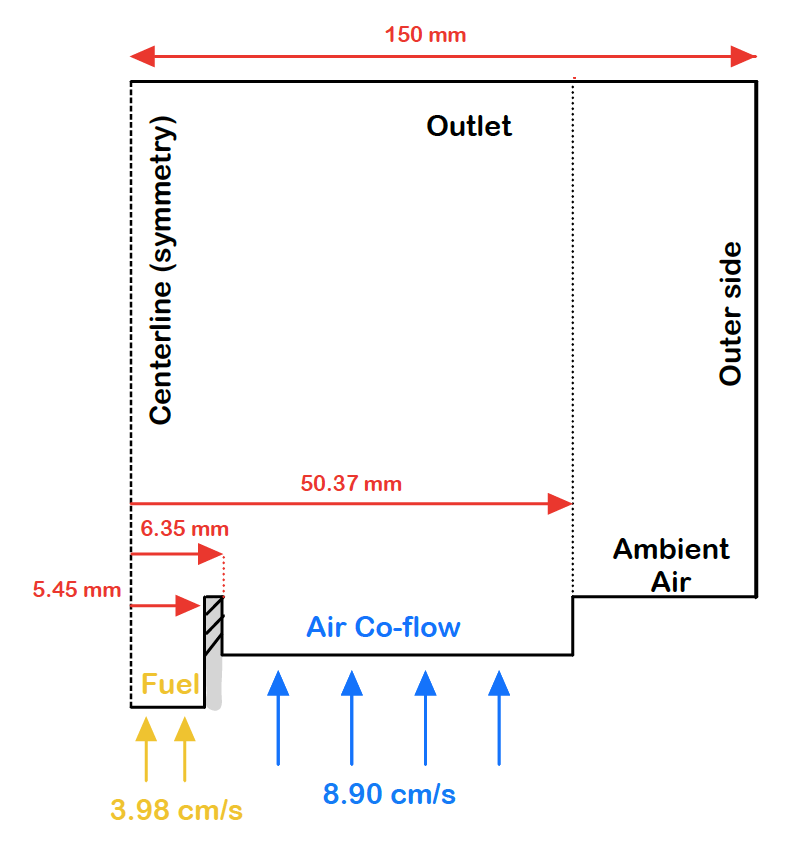
\includegraphics[width=\textwidth]{figures/meshes/SantoroBurnerLiterature_meshDiagram_wMeas.png}
         \caption{\emph{Original} Santoro burner}
     \end{subfigure}
     \hfill
     \begin{subfigure}[b]{0.48\textwidth}
         \centering
         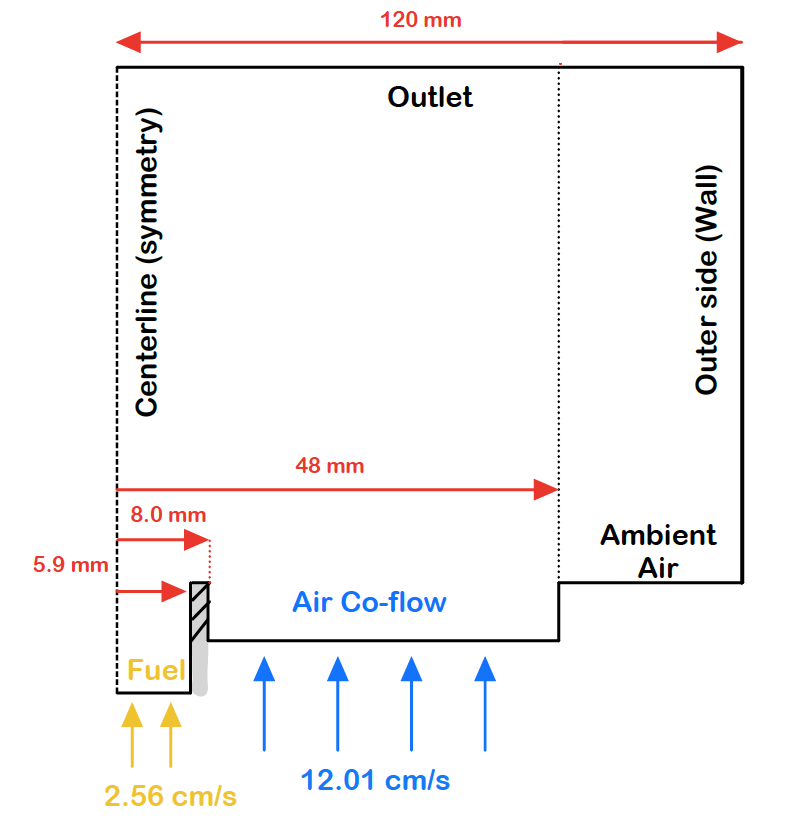
\includegraphics[width=\textwidth]{figures/meshes/fmGlobal_meshDiagram_fuelNozzleMeas.png}
         \caption{\emph{Modified} Santoro burner}
     \end{subfigure}
        \caption{Configurations of the (a)~\emph{original} Santoro burner and (b) the~\emph{modified} Santoro burner with labeled boundaries.}
        \label{fig:meshes}
\end{figure}

% DISCUSS: differences in the meshes and flow conditions
The secondary flame is referred to as the \emph{modified} Santoro burner flame. FM Global\footnote{~\citet{fmGlobal} personal communications.} experimentally studies this flame and provides experimental measurements of the key combustion-related parameters and soot. The flame is very similar to the \emph{original} Santoro burner flame except for different fuel and coflow flow conditions, along with a larger fuel-tube inner diameter of 11.8~mm and a smaller coflow tube of 48~mm inner diameter. Fig.~\ref{fig:meshes} shows a diagram of the two burner's computational domains with corresponding boundaries, radial measurements and flow conditions of the ethylene fuel and air. 

A 30~mm long fuel nozzle is utilized in both configurations to ensure a uniform velocity profile with laminar flow at the exit of the fuel nozzle. A symmetry centerline boundary condition is implemented along with cyclic boundary conditions at the front and back faces of the mesh to utilize the symmetrical geometry of the flame and burner. A linear temperature boundary condition from 400~K to 300~K is prescribed on the fuel nozzle wall to account for fuel pre-heating and demonstrates improved predictions of temperature and species scalar fields~\citep[]{Squeo2021,Dasgupta2015}. Table~\ref{table:flames_flow_conditions} summarizes the flow conditions for the two target 2D ethylene/air flames on the two slightly modified burners. Due to the varying flow conditions and modified burner geometry, both flames have slightly different shapes, flame heights, radiative fluxes and prediction of key-parameters. The convective time is calculated as the ratio of the flame height to the averaged velocity between the fuel and air streams for each flame, respectively.

% TABLE: Santoro vs FM Global flame flow conditions
\begin{table}[H]
\centering
\captionsetup{justification=centering}
\caption{Flow conditions for the two target coflow laminar diffusion flames.}
 \begin{tabular}{ c  c  c } 
 \hline 
 Case & \textbf{Original Santoro burner} & \textbf{Modified Santoro burner} \\
 \hline \hline
 Fuel & Ethylene (C\textsubscript{2}H\textsubscript{4}) & Ethylene (C\textsubscript{2}H\textsubscript{4}) \\ %\hline
 Oxidizer & Air & Air \\ %\hline
 Fuel flow rate & 3.85~cm\textsuperscript{3}/s & 2.80~cm\textsuperscript{3}/s  \\ %\hline
 Fuel velocity & 3.98~cm/s & 2.56~cm/s \\ %\hline
 Oxidizer flow rate & 713.3~cm\textsuperscript{3}/s & 1083.0~cm\textsuperscript{3}/s \\ %\hline
 Oxidizer velocity & 8.90~cm/s & 12.01~cm/s \\ 
 Convective time & 0.70 s & 0.62 s \\
 \hline
 \end{tabular}
\label{table:flames_flow_conditions}
\end{table}


%\subsection{Baseline simulation results}
% DISCUSS: well-validated converged steady state flame solutions with radial profiles at various heights above the burner predictions close to exp. meas., mesh resolution!
Fig.~\ref{fig:baselineContours} shows the baseline iso-contours of temperature, soot volume fraction and molar fractions of carbon dioxide and hydroxyl radical for the \emph{original} Santoro burner flame. The stoichiometric mixture fraction line is superimposed as the dashed black lines to indicate the location of flame. The overall prediction of flame shape and length is satisfactory. Soot appears in the fuel-rich region of the flame, which is reasonable. Radial profiles of baseline results for both flames are discussed in Sec.~\ref{sec:results} and are available in~\citep[]{Squeo2021}.
%The two 2D ethylene/air coflow laminar diffusion flames at atmospheric pressure are steady flames. 
%Predicted radial profiles at various heights above the burner for both target flames yield very satisfactory agreement with available experimental measurements of temperature, soot volume fraction and species concentrations of hydroxyl, carbon dioxide, carbon monoxide and acetylene~\cite{Squeo2021}. Peak temperature is slightly under predicted by approximately 30~K at heights below the flame tip with a slight shift in the temperature profile such that the radial location of the peak temperature from the flame centerline is not captured entirely. However, radial profiles of predicted temperatures for both flames are well within the reported uncertainty band of measured temperatures, taken to be $\pm10\%$~\cite{Dasgupta2015} for the \emph{original} Santoro burner flame and $\pm5\%$ for the \emph{modified} Santoro burner flame, as reported by our collaborators at FM Global. The shift in the temperature profile can be an affect of the skeletal LYR32 chemical mechanism, the two-equation soot model employed and/or thermal boundary conditions of the fuel nozzle. 

% FIGURE: Baseline contours T, sootFv, CO2, OH for the original Santoro flame
\begin{figure}[H]
     \centering
     \begin{subfigure}[b]{0.245\textwidth}
         \centering
         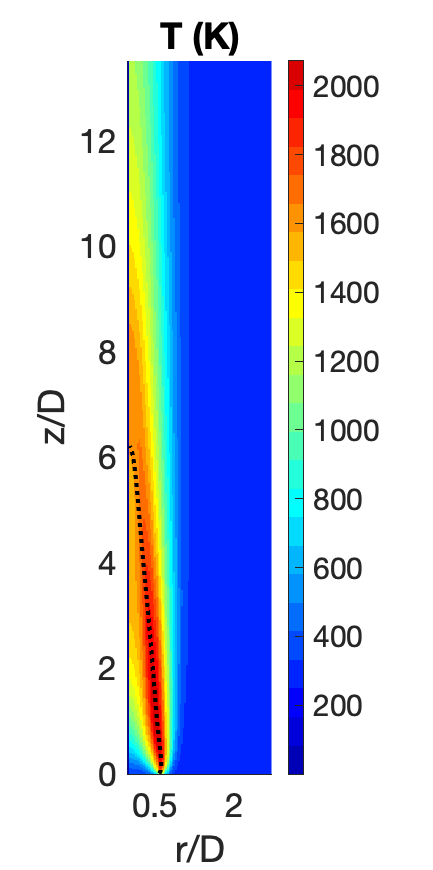
\includegraphics[width=\textwidth]{figures/santoro/Tcontour.png}
         \caption{Temperature}
     \end{subfigure}
     \hfill
     \begin{subfigure}[b]{0.25\textwidth}
         \centering
         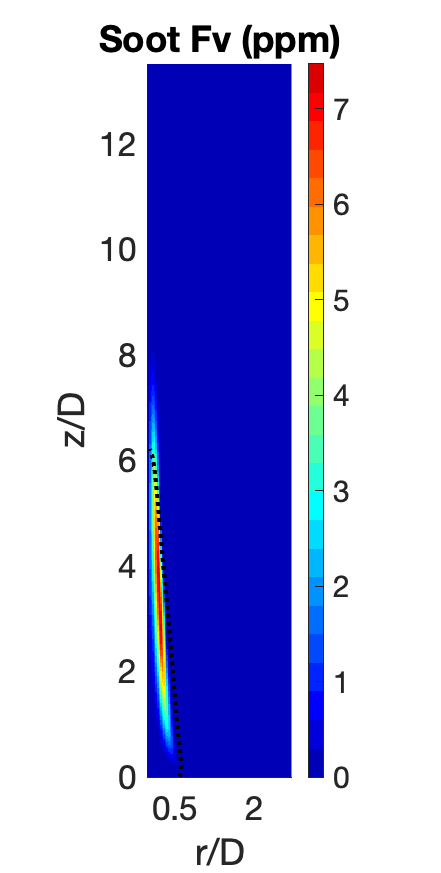
\includegraphics[width=\textwidth]{figures/santoro/fvContour.png}
         \caption{Soot volume fraction}
     \end{subfigure}
     \begin{subfigure}[b]{0.245\textwidth}
         \centering
         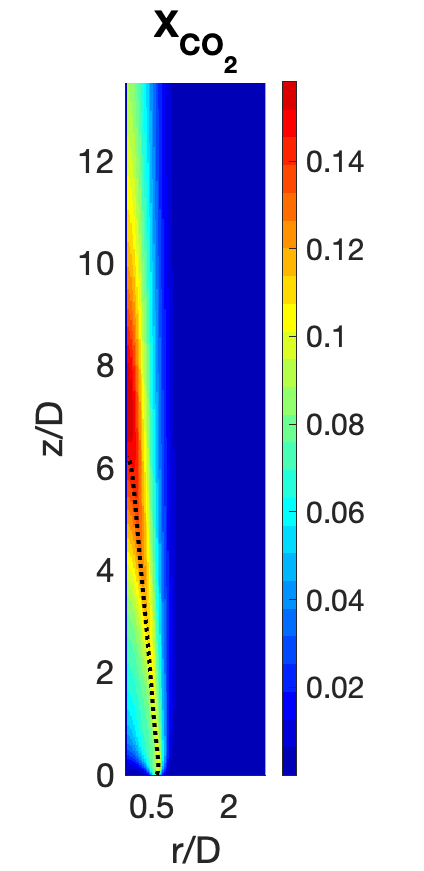
\includegraphics[width=\textwidth]{figures/santoro/CO2Contour.png}
         \caption{CO\textsubscript{2} mole fraction}
     \end{subfigure}
     \begin{subfigure}[b]{0.215\textwidth}
         \centering
         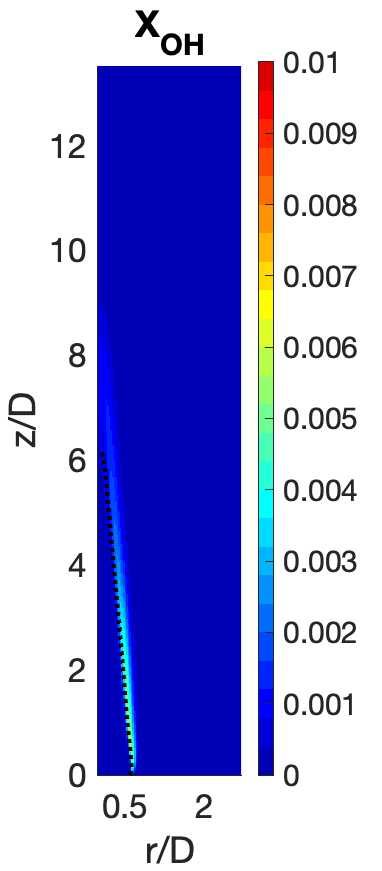
\includegraphics[width=\textwidth]{figures/santoro/OHcontour.png}
         \caption{OH mole fraction}
     \end{subfigure}
        \caption{2D iso-contours of the converged baseline solution for the laminar ethylene/air diffusion flame on the \emph{original} coflow Santoro burner. The dotted black line represents the stoichiometric mixture fraction.}
        \label{fig:baselineContours}
\end{figure}
% DO WE NEED CONTOURS OF THE FM GLOBAL FLAME BASELINE SOLUTION TOO? I DID REFER TO MY THESIS

% DISCUSS: contours, flame height/shape prediction, fuel nozzle boundary condition affect
%Peak soot volume fraction is slightly overpredicted within the flame and under predicted near the tip of the flame. Overall, the shape of the soot profile is predicted sufficiently well, although the location of the profile is predicted closer towards the flame centerline as compared to the laser induced incandescence (LII) experimental measurements with reported uncertainties upwards of $\pm20\%$ for both flames. Acetylene, carbon monoxide, carbon dioxide and hydroxyl are all predicted within the uncertainty bands, taken to be $\pm20\%$ and $\pm50\%$ for hydroxyl radical. 








% ======================================================= %
\section{Results and discussions} \label{sec:results}

\subsection{1D machine learning}
% DISCUSS: the 1D premixed ethylene/air flames from Somesh Roy, chem. mechanisms, soot model variants, well-validated
The potential of the machine learning regression model to predict soot volume fraction in flames is first demonstrated in simple 1D premixed flames. Datasets containing well-validated numerical solutions to five 1D premixed ethylene/air flames are provided by Somesh Roy~\citep[]{Roy_Haworth,Roy}. A laminar premixed ethylene/air flame~\citep[]{Kazakov1995} at atmospheric pressure and a carbon-to-oxygen ratio of 0.69 is chosen as it is most similar to the 2D target ethylene/air flames tested in this work.

%\subsubsection{Regression model training.}
% DISCUSS: Regression training, jw1.69 flame, chem. mech., soot models, penalty coeff
Initially, the Poisson regression model is trained on a set of key combustion parameters deemed to have the largest impact on soot prediction. These parameters, known to affect soot evolution processes, include temperature and species concentrations of C\textsubscript{2}H\textsubscript{2},~O\textsubscript{2},~O,~OH,~H\textsubscript{2} and the corresponding soot volume fractions~(F\textsubscript{v}) from a particular flame solution. An optimal penalty coefficient of $\alpha=0.10$ is used to prevent over and under fitting of the model and determined to yield the best soot prediction quantified with the lowest root mean square error. The root-mean squared error~(RMSE) is utilized to quantify the accuracy of the baseline numerical flame solutions of soot volume fraction and predictions using the trained regression model, where RMSE is expressed as
\begin{equation}
    RMSE = \sqrt{\frac{\sum_{i=1}^N \left(\hat{y}_i-y_i\right)^2}{N}} \\ 
    \label{eq:RMSE}
\end{equation}
where $N$ is the number of discrete points, $\hat{y}_1,\hat{y}_2,\dots,\hat{y}_N$ are predicted values and $y_1,y_2,\dots, y_N$ are observed values.

The model is trained using 1D numerical flame results from five different chemical mechanisms: WF99~\citep[]{Wang1997}, USCII~\citep[]{Wang2007_USCII_mech}, ABF100~\citep[]{Appel2000}, QLY33~\citep[]{Mehta2009}, and SF93~\citep[]{Slavinskaya2009} and tested on the remaining ABF31~\citep[]{Mehta2009} mechanism. ABF31 is chosen as the test mechanisms as it produced a peak soot concentration that is well within the range of the minimum and maximum peak soot concentrations of the chemical mechanisms in the training dataset. 
%It is important for the training flame data to be as similar to the target flame as possible. The training data should contain the entire range of soot concentrations in the target flame or else the model risks missing soot concentrations in the target flame that are not covered in the training data. 

% FIGURE: 1D scatter plot of soot vs. ln(T) 
\begin{figure}[!ht]
\begin{center}
\makebox[\textwidth][c]{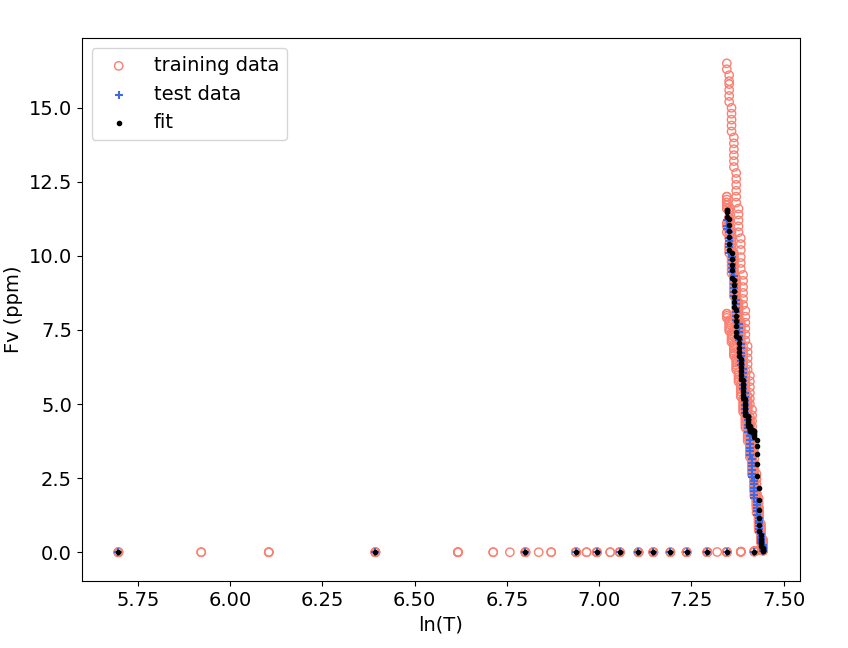
\includegraphics[width=0.6\textwidth]{figures/machLearning/JW1.69_train2Eq_testABF31mesh_poisson.png}}
\end{center}
\caption{Soot volume fraction vs. the natural logarithm of temperature for the training and testing datasets along with the prediction from the trained Poisson regression model for the 1D laminar premixed flame. A modified two-equation soot model is used to generate the data.}
\label{fig:1D_machLearning}
\end{figure}

%\begin{figure}[!ht]
%     \centering
%     \begin{subfigure}[b]{0.495\textwidth}
%         \centering
%         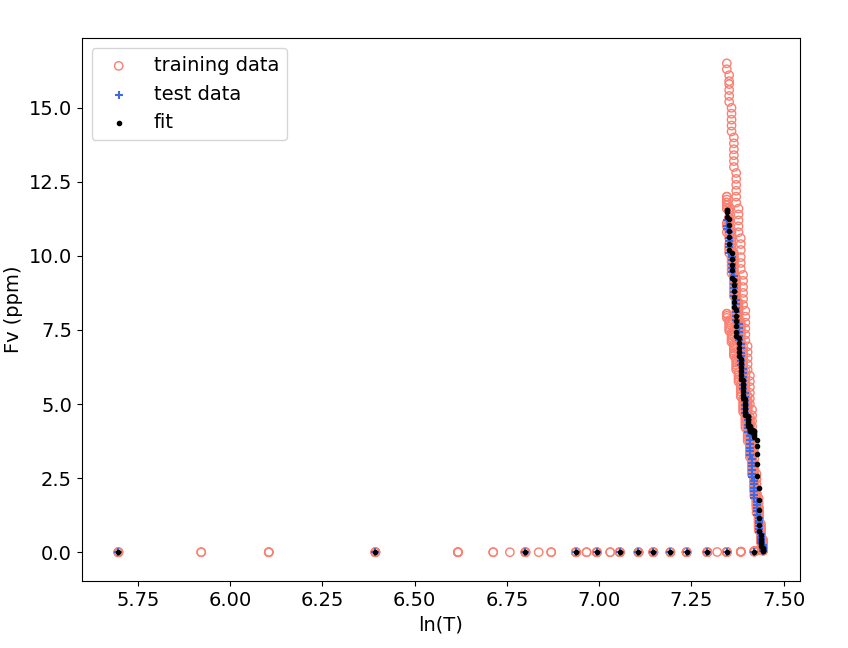
\includegraphics[width=\textwidth]{figures/machLearning/JW1.69_train2Eq_testABF31mesh_poisson.png}
%         \caption{Two-Equation soot model}
%     \end{subfigure}
%     \hfill
%     \begin{subfigure}[b]{0.49\textwidth}
%         \centering
%         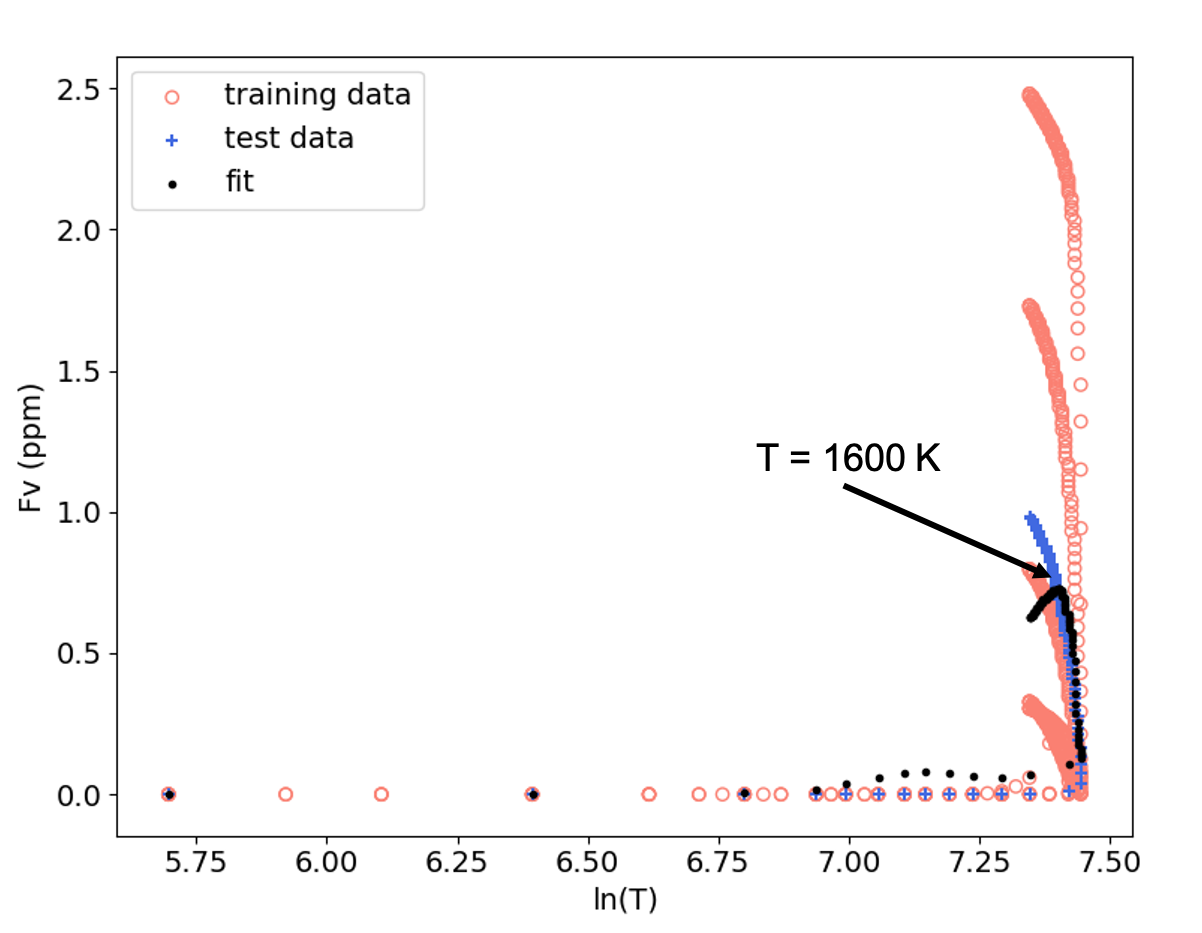
\includegraphics[width=\textwidth]{figures/machLearning/inflectionPointTemp_JW1.69_DSMTrain_testABF31.png}
%         \caption{DSM soot model}
%     \end{subfigure}
%     \caption{Soot volume fraction vs. the natural logarithm of temperature for the training and testing datasets along with the prediction from the trained Poisson regression model for the 1D laminar premixed flame. A modified two-equation soot model is used to generate the data in (a) and the discrete sectional soot model is used in (b).}
%        \label{fig:1D_machLearning}
%\end{figure}

% DISCUSS: scatter plots of soot vs. ln(T), fits, inflection point at T=1600K as peak soot formation where transition from inception to surface growth reactions (Smooke's paper), residency time of soot (need velocity/strain rates)
The regression model is trained entirely from a numerical flame solution produced with the two-equation soot model~\citep[]{Leung_Lindstedt_Jones} tuned to premixed flames using the C/O ratio of the flame~\citep[]{Roy}.
%, then with a numerical flame solution produced using the high-fidelity discrete sectional soot model~\citep[]{Roy}. 
Fig.~\ref{fig:1D_machLearning} shows the training, testing and predicted fit of soot volume fraction plotted against the natural logarithm of temperature for the trained Poisson regression model for the 1D premixed flame. Soot predicted by the trained model yields a very accurate fit with a RMSE of 0.09~ppm when compared to the test dataset. 
% while the model trained with the discrete sectional soot model results yields a RMSE of 0.16~ppm. 
RMSE is a measure of the standard deviation of the distribution of errors for the predicted fit against the test dataset. A smaller RMSE indicates the predicted fit is very close to the test dataset yielding a very accurate prediction of the soot field.
%An inflection point in the soot prediction is observed at a temperature of 1600~K in Fig.~\ref{fig:1D_machLearning}(b), below which the regression diverges from the test data. Soot formation processes begin in flames near temperatures around 1300~K and peaks at temperatures of about 1600~K~\citep[]{Turns}.
%At this temperature, primary soot particle growth shifts from an inception dominant process to a surface growth dominant process.
%Since the model's training dataset does not include parameters of the flow field or flame speed, the transport of initially formed soot particles cannot be captured. As a result, at temperatures below 1600~K, the model cannot accurately predict the entire soot field of the target dataset due to the transport of soot particles in the flame.




\subsection{2D machine learning}
% DISCUSS: the objective of 2D flame prediction (train on one flame, predict similar flame), streamline extraction
After successfully training and testing the regression model on 1D flames, the methodology is extended to 2D laminar diffusion flames. The model is first trained and tested on the \emph{original} Santoro burner flame to verify the predicted solution and model. Then the model is trained on one of the flame datasets at a time and tested on the remaining flame. Streamlines are extracted from the computational flame in a pre-processing step such that the discrete scalar fields can be obtained from the flame to build the training and testing datasets. Due to the computational burden associated with most numerical flame solvers, the ultimate goal is to predict the soot field in a target flame outside of the training data with a regression model trained on a series of well-validated flame solutions. Ultimately, the regression model can be trained on one of these small-scale simple laminar flames then tested on larger turbulent pool-fires that are much more computationally expensive to numerically simulate and predict soot concentrations accurately.

\subsubsection{Regression model training.}
% DISCUSS: training on original santoro flame, predict FM Global flame then vice-versa, choice  of model parameters, penalty coefficient
The Poisson regression model is trained on an optimal set of key combustion parameters affecting soot evolution processes, based on the work of~\citet{Zimmer2019} and a parametric study conducted in~\citep[]{Squeo2021}, with some results discussed in Sec.~\ref{sec:paramtericStudy}. These parameters include temperature, streamwise and radial velocities, strain rate and species concentrations of C\textsubscript{2}H\textsubscript{2}, H\textsubscript{2}, O\textsubscript{2}, O, OH, CO\textsubscript{2} and the corresponding soot volume fractions from a particular flame solution. Velocities and strain rates are used to train the model to capture both the transport of soot particles and the residence time of soot in the flame.~\citet{Smooke2005} showed that soot formation depends on the fluid dynamic residence time, where soot concentration increases significantly after 15-20~ms in atmospheric, nonpremixed, coflowing laminar flames.

A variable penalty coefficient is used depending on the type of training and testing data. When the training data covers the entire range of soot volume fractions in the target test flame dataset, a large penalty coefficient of $\alpha=0.10$ is suitable to prevent over fitting by penalizing complex model coefficients. When the testing data contains soot concentrations outside of the training data, such that extrapolation is required to capture the soot field in the test flame, then a smaller penalty of $\alpha=0.001$ is used to allow for a slightly over fit model. In this work, a smaller penalty of $\alpha=0.001$ is found to yield the best soot prediction when training and testing the model on separate streamlines from the same flame.

% DISCUSS: describe training for scatter plots
First, the model is trained on the \emph{original} Santoro burner flame and tested on the same flame. A dataset is generated from 100 streamlines extracted from the flame that originate at the burner surface and follow the streamwise flow to the top of the computational mesh. Training and testing datasets are determined by splitting the 100 streamline dataset into 70$\%$ for the training data and the remaining 30$\%$ for testing such that both datasets are independent of one another. Results of the training data, testing data and predicted regression fit of soot volume fraction as a function of the natural logarithm of temperature for the 2D laminar ethylene/air atmospheric flame on the \emph{original} Santoro burner are shown in Fig.~\ref{fig:2D_soot_v_lnT_scatterPlots}(a). The model is then trained on all 100 streamlines from the \emph{original} Santoro burner flame and tested on 100 streamlines extracted from the \emph{modified} Santoro burner flame. Soot concentrations predicted by the regression model for the \emph{modified} Santoro burner flame, along with the training and testing soot concentrations, are shown in Fig.~\ref{fig:2D_soot_v_lnT_scatterPlots}(b).

% FIGURE: 2D scatter plot of soot vs. ln(T) for both flames
\begin{figure}[H]
     \centering 
     \begin{subfigure}[b]{0.49\textwidth}
         \centering
         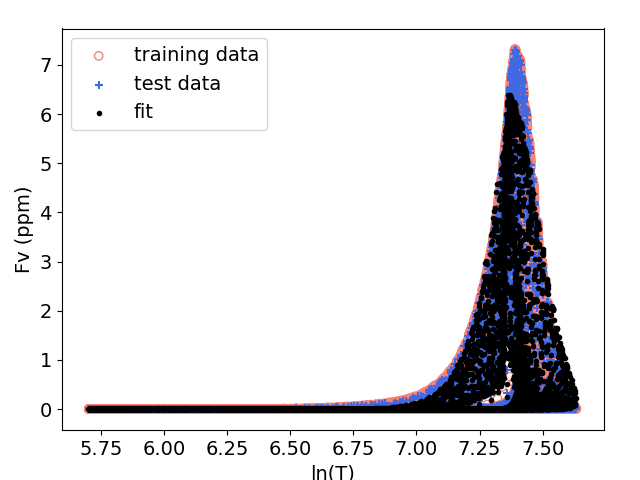
\includegraphics[width=\textwidth]{figures/machLearning/trainSantoro_testSantoro_alpha0.001._deg2.png}
         \caption{Train and test on the \emph{original} burner flame}
     \end{subfigure}
     \hfill
     \begin{subfigure}[b]{0.49\textwidth}
         \centering
         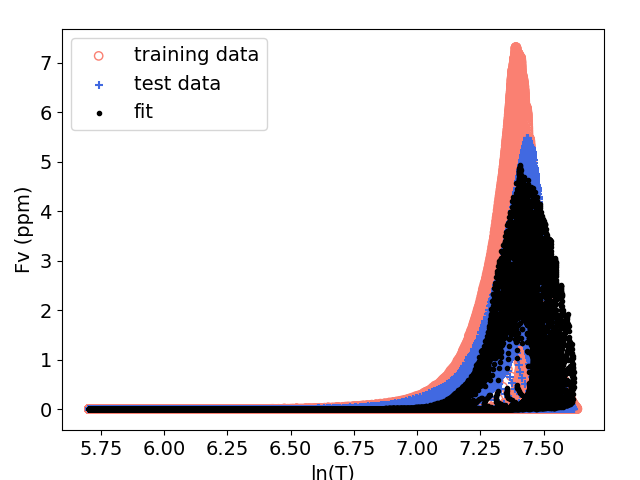
\includegraphics[width=\textwidth]{figures/machLearning/trainSantoro_testFM_alpha0.1._deg2.png}
         \caption{Train on the \emph{original} burner flame, test on the \emph{modified} flame}
     \end{subfigure}
        \caption{Soot volume fraction versus the natural logarithm of temperature for the training and testing datasets along with the prediction from the trained Poisson regression model for the 2D laminar diffusion ethylene/air flame: (a) the model is trained and tested on separate streamlines from the \emph{original} burner flame with $\alpha=0.001$ and (b) the model is trained on the \emph{original} burner flame and tested on the \emph{modified} burner flame with $\alpha=0.10$.}
        \label{fig:2D_soot_v_lnT_scatterPlots}
\end{figure}

% DISCUSS: explain scatter plot results and introduce/explain contour plots
The trained regression model is capable of capturing the location of soot in the flame and the magnitude of soot concentration reasonably well in both flames tested. Peak soot concentrations are missed by approximately 1~ppm, although the location and structure of the peak are well predicted. The model prediction, when trained on the \emph{original} Santoro burner flame and tested on streamlines from the same flame, yields a RMSE of 0.32~ppm. When the model is trained on the \emph{original} Santoro burner flame then used to predict the soot field in the \emph{modified} Santoro burner flame, the model yields a RMSE of 0.28~ppm.
%Hence, the error of soot volume fraction predicted by the regression model compared to the actual testing dataset has a standard deviation of 0.28 ppm. 

Fig.~\ref{fig:2D_contoursSantoro} shows iso-contours of the soot field in ppm for (a) the baseline numerical solution from \texttt{OpenFOAM} without any regression, (b) the testing data of the \emph{original} burner flame and (c) the regression prediction of the soot field in the same \emph{original} burner flame. Fig.~\ref{fig:2D_contoursFM} shows similar iso-contours of the soot field in ppm, except for the (a) baseline solution for the \emph{modified} Santoro burner flame, (b) the training dataset from the \emph{original} burner flame and (c) the resulting regression prediction of the \emph{modified} burner flame. Ideally, the regression model prediction in contour (c) should replicate the baseline contour in (a). Overall, the location and structure of the soot field in the flames are well captured, although the magnitude of peak soot concentration is not fully resolved with an approximate difference of 1 ppm. The fit of the regression model can be controlled with the penalty coefficient, $\alpha$, which determines if the regression model will under or over fit the test dataset. In this sense, a highly over fit model can be used to reduce the overall RMSE of the fit and better capture the peak soot concentrations. However, the resulting model coefficients $\mathbf{w}$ in Eq.~\ref{eq:objectiveFunctionPoisson} will be very complex and susceptible to numerical error in calculations.

% FIGURE: contours of soot, train on original Santoro and test on same flame
\begin{figure}[!ht]
\begin{center}
\makebox[\textwidth][c]{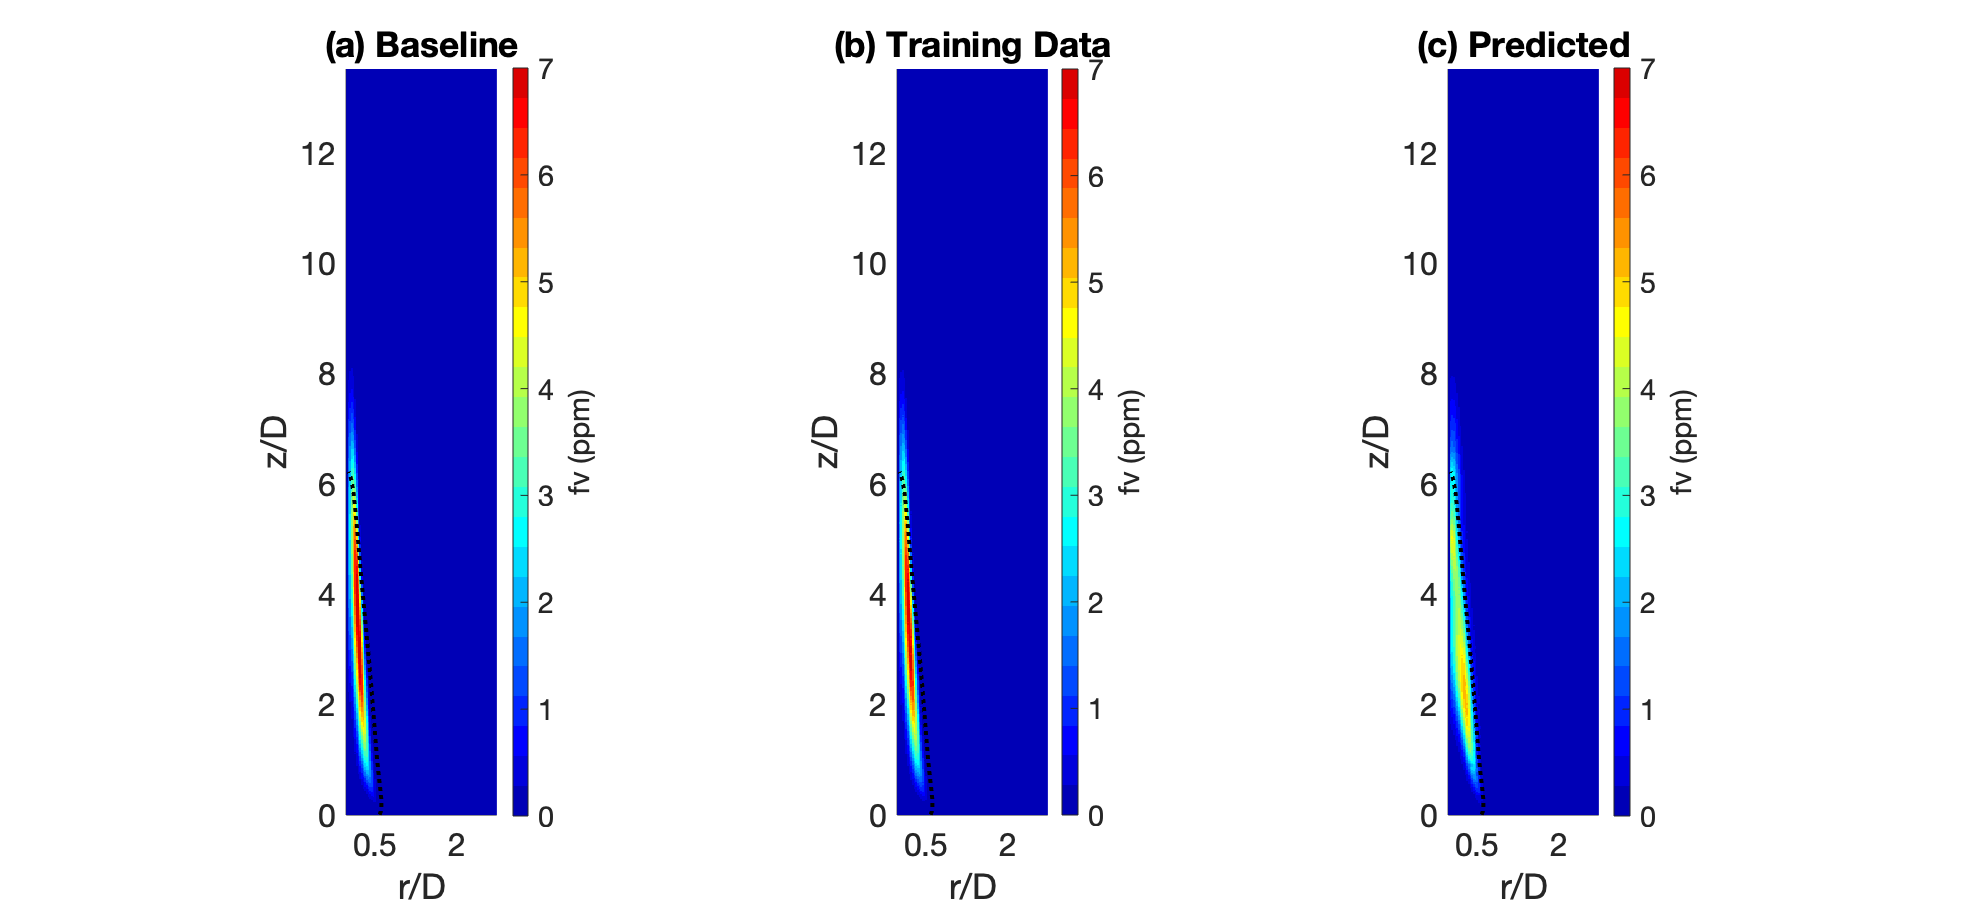
\includegraphics[width=0.8\textwidth]{figures/machLearning/predictSantoro_100streamlines_contours.png}}
\end{center}
\caption{Iso-contours of soot volume fraction (ppm) for (a) the baseline \emph{original} Santoro burner coflow flame, (b) the training data from the \emph{original} Santoro burner coflow flame and (c) and the regression prediction of the same flame. Poisson regression with a penalty coefficient $\alpha=0.001$ and a second degree nonlinear feature space mapping is used.}
\label{fig:2D_contoursSantoro}
\end{figure}

% FIGURE: contours, train using original Santoro, predict FM flame
\begin{figure}[!ht]
\begin{center}
\makebox[\textwidth][c]{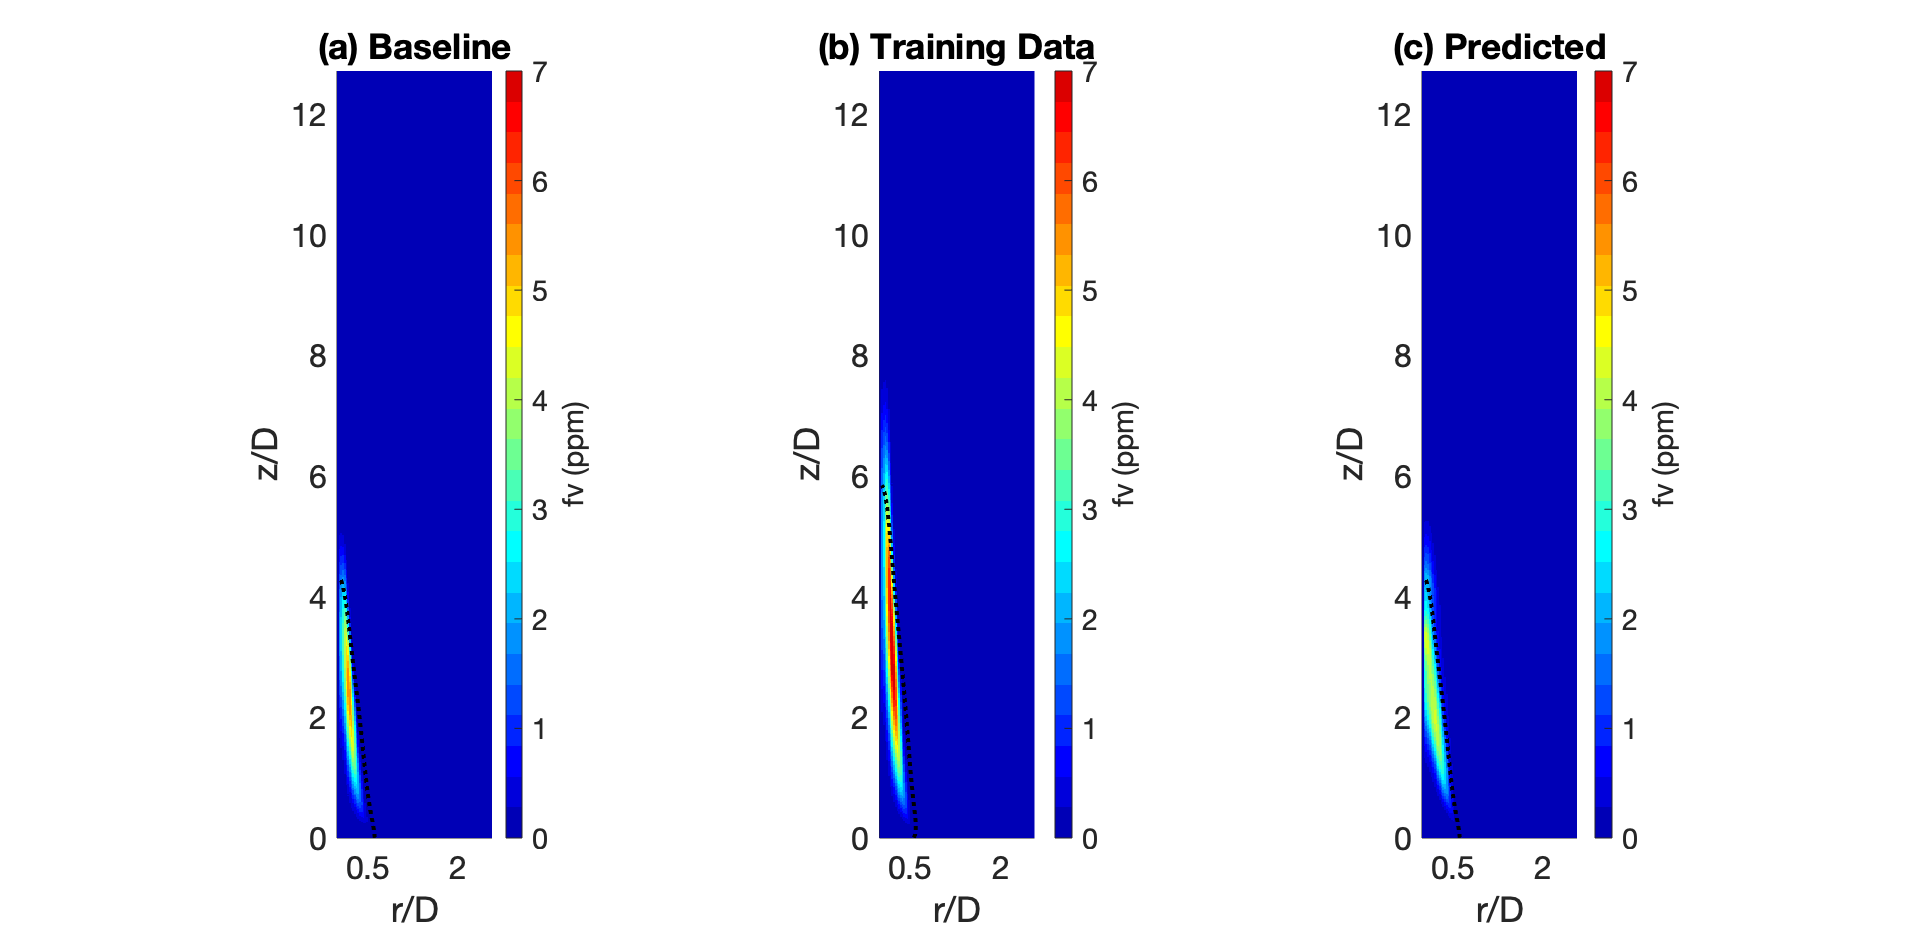
\includegraphics[width=0.8\textwidth]{figures/machLearning/predictFM_100streamlines_contours.png}}
\end{center}
\caption{Iso-contours of soot volume fraction (ppm) for (a) the baseline \emph{modified} Santoro burner coflow flame, (b) the training data from the \emph{original} Santoro burner coflow flame and (c) and the regression prediction of the \emph{modified} burner flame. Poisson regression with a penalty coefficient $\alpha=0.10$ and a second degree nonlinear feature space mapping is used.}
\label{fig:2D_contoursFM}
\end{figure}

% DISCUSS: radial profile line plots, improvement of regression prediction due to slight underprediction of flame soot concentrations
Radial profiles of the predicted and baseline soot volume fraction in ppm at various heights above the burner are compared against experimental measurements with an estimated uncertainty\footnote{Experimental measurements and uncertainties are obtained through personal communications with collaborators at FM Global~\citep[]{fmGlobal}.} of $\pm20\%$, as shown in Fig.~\ref{fig:soot_linePlot}. The regression model is trained on the \emph{original} Santoro burner flame then tested on the \emph{modified} burner flame. The baseline solution over predicts soot at every height above the burner, while the regression predicted solution adjusts towards experimental measurements. One explanation for the improved regression prediction of soot compared to the baseline is that the regression model does not fully capture peak soot concentrations in the target flame, resulting in a slight under prediction of soot at all regions in the flame such that the prediction is closer to experimental measurements. Nonetheless, the regression model shows promise to predict soot volume fraction with comparable accuracy as the baseline CFD model. 

% FIGURE: FM Global HAB line plots for exp., baseline, regression prediction
\begin{figure}[!ht]
\begin{center}
\makebox[\textwidth][c]{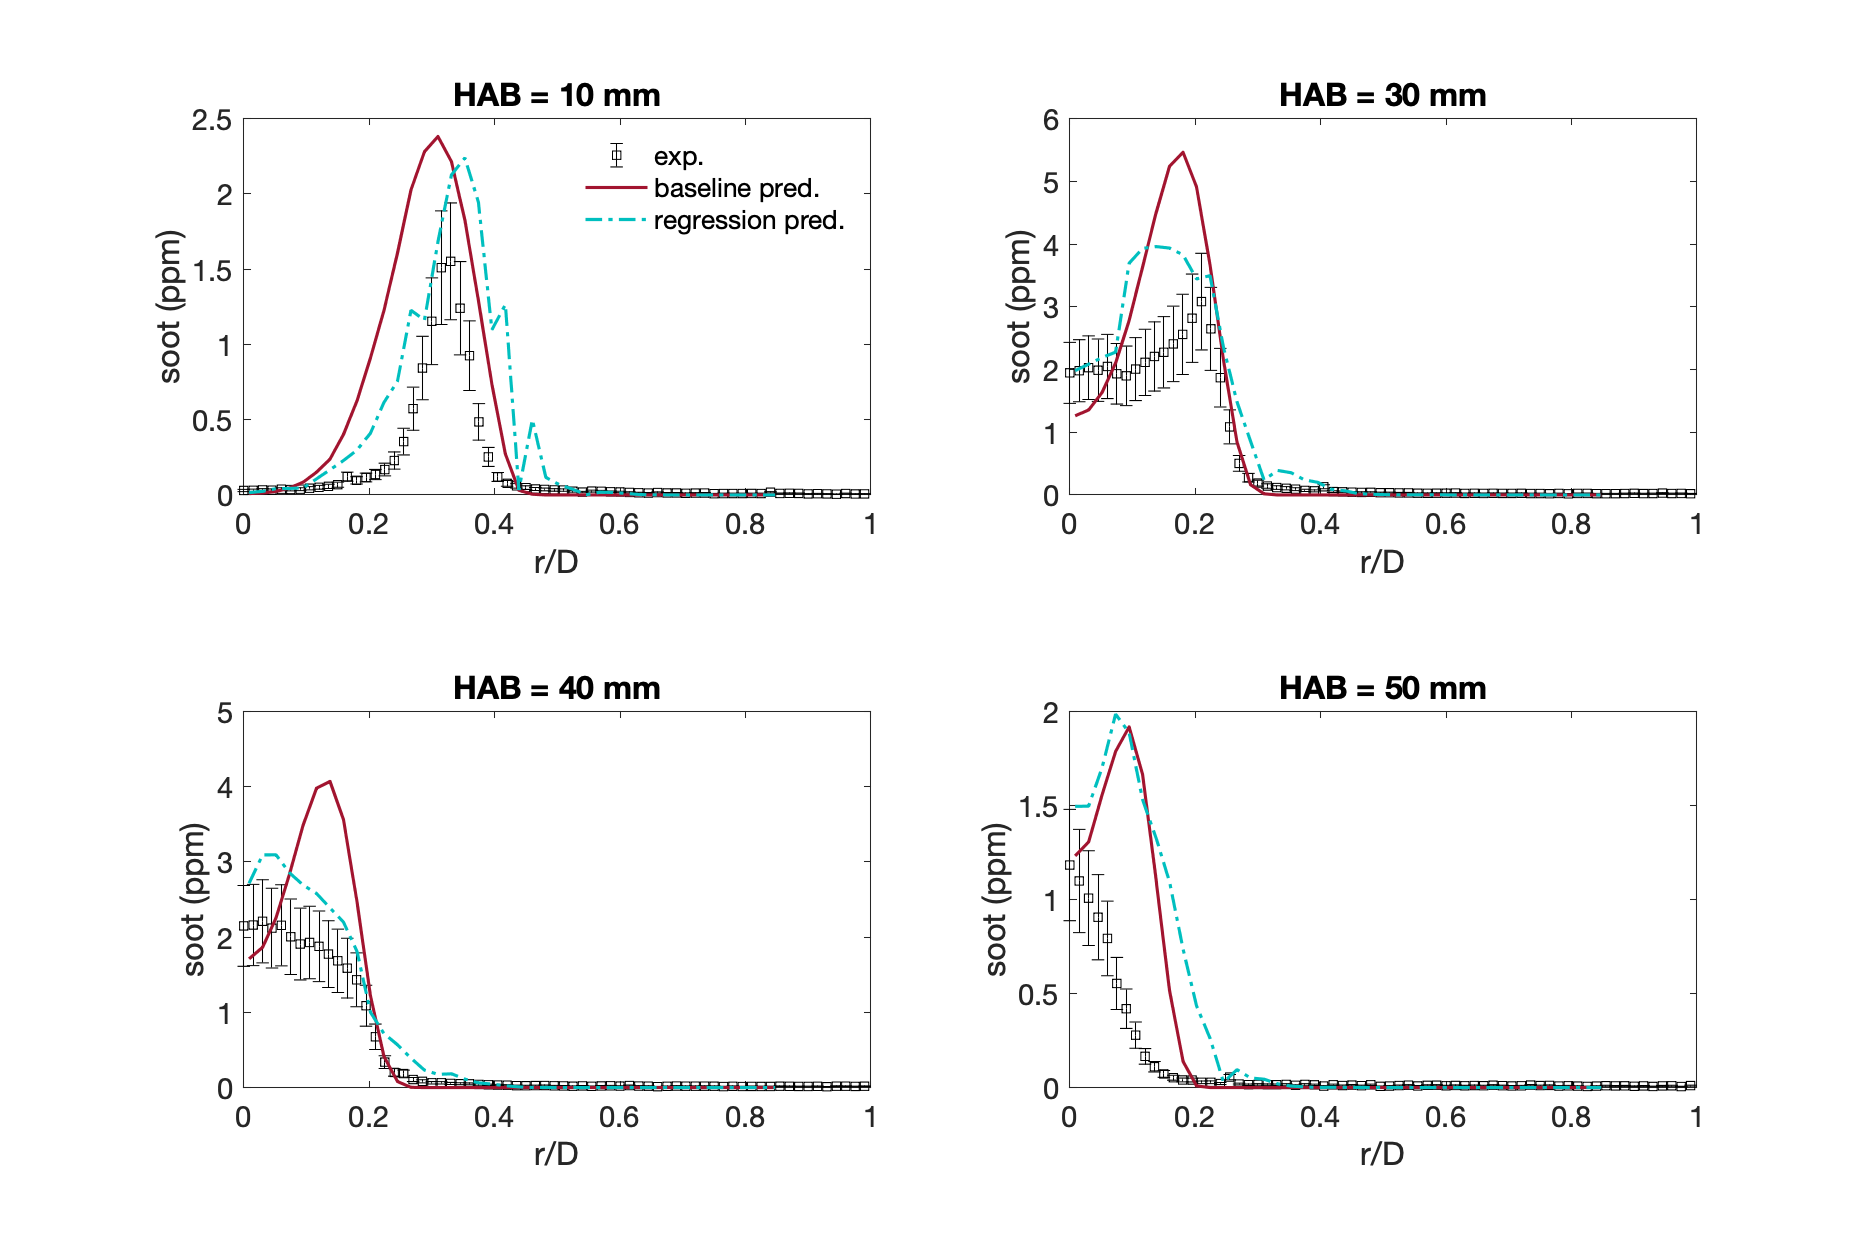
\includegraphics[width=0.9\textwidth]{figures/machLearning/soot_linePlot_fmGlobal_exp__baseline_machLearn.png}}
\end{center}
\caption{Soot volume fraction (ppm) radial profiles at various heights above the burner for the 1-bar C\textsubscript{2}H\textsubscript{4}-air laminar diffusion flame on the \emph{modified} Santoro burner using
the two-equation soot model and LYR32 chemical mechanism. Experimental measurements~\citep[]{fmGlobal} (exp.) are plotted against the baseline simulation solution and regression prediction of soot.}
\label{fig:soot_linePlot}
\end{figure}






\subsubsection{Cross validation.}
% DISCUSS: train on fm flame data, test original santoro burner flame
% DISCUSS: better fit training with Santoro and testing on modified burner flame (due to smaller flame and more soot?)
In another test, the regression model is trained on streamline data from the \emph{modified} Santoro burner flame and tested on the \emph{original} Santoro burner flame. Since the training flame now has a lower peak soot volume fraction than the test flame, the regression model predicts the structure of soot adequately well but cannot capture the magnitude of peak soot concentrations in the \emph{original} Santoro burner flame well when a penalty coefficient of $\alpha=0.10$ is applied. When the penalty coefficient is reduced to $\alpha=0.001$ to allow for over fitting, the regression model is able to capture the peak soot concentrations sufficiently well with a RMSE of 0.44 ppm. Comparatively, when the larger penalty coefficient of $\alpha=0.10$ is used, the prediction yields a RMSE of 0.85 ppm. A smaller penalty coefficient is required when the range of soot concentrations in the training data does not cover the range of soot in the target flame. In general, when testing the regression model on flames with unknown soot concentrations, as long as the training data is well-validated and sufficiently close to the target flame, a penalty coefficient of $\alpha=0.001$ is found to yield the best soot prediction to maximize the reduction of error between the discrete training and testing data.

% DISCUSS: RMSE table and better prediction training on original Santoro than FM flame
Table~\ref{table:RMSE_exp_baseline_machLearn} displays the RMSE of both 2D diffusion flames tested for (1) the baseline numerical solution from \texttt{OpenFOAM} and (2) the predictions of soot from the trained regression model. RMSE of both the baseline solution and trained model prediction of soot are computed against available experimental measurements of soot volume fraction throughout the flame at various heights above the burner using Eq.~\ref{eq:RMSE}. The regression prediction for the original Santoro burner is produced by training the model using the \emph{modified} Santoro burner flame solution and testing on the \emph{original} Santoro burner flame and vice-versa for the \emph{modified} Santoro burner. Overall, the baseline solution of the \emph{modified} Santoro burner flame is better predicted than the \emph{original} Santoro burner flame.
 
Regression prediction of soot in the \emph{original} Santoro burner flame, when trained on the \emph{modified} Santoro burner flame, does not improve the RMSE when compared against available experimental measurements of soot. This is a consequence of the training datasets. Fig.~\ref{fig:2D_soot_v_lnT_scatterPlots} shows that the \emph{original} Santoro burner flame has a greater peak soot concentration than the \emph{modified} burner flame. %Therefore, the regression model cannot capture soot concentrations in this peak when trained on the \emph{modified} burner flame as these soot concentrations are not captured in this flame's training data. In order to achieve accurate prediction of the entire soot field in a target flame using the procedure presented, the regression model should be trained on a dataset containing the entire range of soot concentrations in the target test flame.
Therefore, the regression model cannot capture soot concentrations in this peak when trained on the \emph{modified} burner flame as these soot concentrations are not captured in this flame's training data. Using a penalty coefficient near zero or equal to zero allows for an over fit model that can extrapolate data such that an accurate prediction of the entire soot field in a target flame is achieved~\citep[]{Squeo2021}. However, the regression model should be trained on a dataset generated from a flame most similar to the target test flame for the most accurate prediction. 

% TABLE:  RMSE of predictions vs. exp. measurements
\begin{table}[!ht]
\centering
\captionsetup{justification=centering}
\caption{Root mean squared error (ppm) between available experimental measurements and the (1)~baseline solution and (2)~regression prediction of soot volume fractions.}
 \begin{tabular}{ c  c  c } 
   & \textbf{Original Santoro burner} & \textbf{Modified Santoro burner} \\
 \hline \hline
(1) Baseline solution & 1.73 & 0.65 \\ \hline
 
(2) Regression prediction & 1.78 & 0.50 \\ \hline

 \end{tabular}
\label{table:RMSE_exp_baseline_machLearn}
\end{table}





\subsubsection{Parametric study.} \label{sec:paramtericStudy}

% DISCUSS:   optimal model parameters 
A set of parameters including temperature, mixture fraction, radial and streamwise velocities and mass fractions of acetylene, monotonic oxygen, diatomic oxygen, hydroxyl radical, diatomic hydrogen and carbon dioxide, is employed in the regression model above. A parametric study is conducted here on the optimal set of parameters relating to combustion and soot evolution processes to obtain the most accurate trained model prediction of soot volume fraction. The model is trained and tested on streamline datasets from the \emph{original} Santoro burner flame and all other factors are kept constant in each training combination, including the penalty coefficient $\alpha=0.10$. Table~\ref{table:parameterCombinations} presents a brief overview of the sets of parameter combinations for the input feature space used to train the regression model, ranked in order of most accurate to least accurate with corresponding root-mean square errors. A full parametric study is available in~\citep[]{Squeo2021}. In general, a larger set of training parameters yields a more accurate regression prediction, although at the cost of increased computational time. Training with velocities and the strain rate reduced the RMSE in every combination of parameters tested. Velocity and strain rate allow the regression model to capture information of the flow field. Removing the minor species, such as Y\textsubscript{H2}, Y\textsubscript{O2}, Y\textsubscript{O}, Y\textsubscript{OH} and Y\textsubscript{CO2} from the optimal training set at the top of Table~\ref{table:parameterCombinations} increased the RMSE to 0.98~ppm from its original value of 0.64~ppm. 

% Model combination table
\begin{table}[!ht]
\centering
\captionsetup{justification=centering}
\caption{Ranked RMSE between baseline solution and regression prediction of soot volume fractions using Poisson regression with a second degree feature space mapping and penalty coefficient $\alpha=0.10$ for various model parameter combinations.}
    \begin{tabular}{ c | c | c }   
    \hline  % adds horizontal line
    Rank & Combination & RMSE (ppm) \\
    \hline \hline
    1 & T,~Y\textsubscript{C2H2},~Y\textsubscript{H2},~Y\textsubscript{O2},~Y\textsubscript{O},~Y\textsubscript{OH},~Y\textsubscript{CO2},~U\textsubscript{r},~U\textsubscript{z},~strain~rate & 0.64 \\
    2 & ~Y\textsubscript{C2H2},~Y\textsubscript{H2},~Y\textsubscript{O2},~Y\textsubscript{OH},~Y\textsubscript{O},~Y\textsubscript{CO2},~U\textsubscript{r},~U\textsubscript{z},~mixF,~strain~rate & 0.65 \\
    3 & T,~Y\textsubscript{C2H2},~Y\textsubscript{H2},~Y\textsubscript{O2},~Y\textsubscript{OH},~Y\textsubscript{CO2},~U\textsubscript{r},~U\textsubscript{z},~mixF,~strain~rate & 0.65 \\
    4 & T,~Y\textsubscript{C2H2},~Y\textsubscript{H2},~Y\textsubscript{O2},~Y\textsubscript{O},~Y\textsubscript{CO2},~U\textsubscript{r},~U\textsubscript{z},~mixF,~strain~rate & 0.65 \\
    5 & T,~Y\textsubscript{H2},~Y\textsubscript{O2},~Y\textsubscript{O},~Y\textsubscript{OH},~Y\textsubscript{CO2},~U\textsubscript{r},~U\textsubscript{z},~mixF & 0.68 \\
    \vdots & \vdots & \vdots \\
    28 & T,~U\textsubscript{r},~U\textsubscript{z},~strain~rate & 1.25 \\
    29 & U\textsubscript{r},~U\textsubscript{z},~strain~rate & 1.34 \\
    30 & T or mixF or Y\textsubscript{C2H2} or \dots & $\ge$ 1.34 \\ 
    \hline
    \end{tabular}
    \label{table:parameterCombinations}
\end{table}











\begin{comment}
% ======================================================= %
\subsection{Influence on radiative characteristics}

% DISCUSS: soot and radiation coupling
Soot is a significant contributor to thermal radiation in fires. The soot and thermal radiation coupling in fires is one of the most complex phenomena involved in fire, and remains an important problem since thermal radiation plays a dominant role in the growth and spread of fires~\citep[]{Beji2008}. Thermal radiation accounts for the majority of overall heat transfer to the ambient surroundings in large scale fires~\citep[]{DeRis1979}. By improving thermal radiation prediction through improved soot modeling, fire simulations can provide the fire engineering community with a new advantageous opportunity to explore and better understand how fires evolve, grow and spread. 

% DISCUSS: frozen field analysis, how the rad heat fluxes are obtained
Using the baseline numerical solution and the regression predicted solution of of soot volume fraction, a ray-filtered frozen field radiation analysis is performed to capture the radiative heat flux at a radial distance $r=13.40$~cm away from the flame centerline to replicate measurements taken with a narrow-slit radiometer. These flames have been shown to be optically thin, where absorption within the flame is negligible~\citep[]{DasGupta2015}. Frozen-field analyses can be performed at any time step, where the RTE is solved without evolving any scalar fields, as compared to a full Monte Carlo ray tracing with line-by-line spectral solution with much greater computational burden. A finite number of rays are chosen based on the mesh size and accuracy desired, and emitted from every cell carrying a fixed amount of energy and unique wavenumber, determined using random number correlations~\citep[]{Wang2007,RenTaoandModest2013,Modest2013}. These rays are then collected on a boundary face at $r=13.40$~cm from the flame centerline, where only rays penetrating the boundary face at a fixed angle matching that of the narrow-slit opening of the radiometer used to collect the heat flux measurements are absorbed. Fig.~\ref{fig:heatFluxes} shows the heat flux solution using the frozen field radiation analysis using both the baseline and regression model numerical solutions of soot volume fraction.

% FIGURE: Radiative heat flux comparisons
\begin{figure}[H]
\begin{center}
\makebox[\textwidth][c]{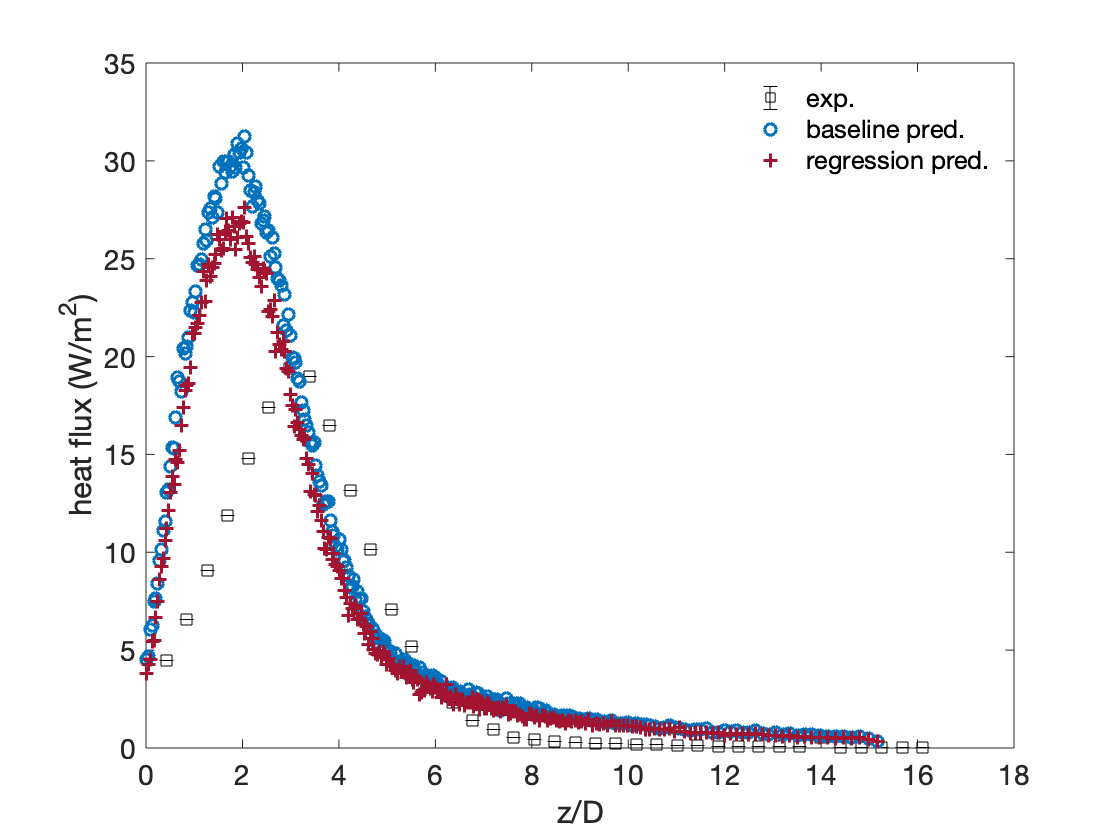
\includegraphics[width=0.7\textwidth]{figures/machLearning/heatFluxesComparison_vs_exp.png}}
\end{center}
\caption{Radiative heat flux (W/m\textsuperscript{2}) measured along the streamwise direction (z) normalized by the fuel tube inner diameter (D). Experimental measurements (exp.) are plotted against the baseline simulation solution and heat flux generated using the regression prediction of soot.}
\label{fig:heatFluxes}
\end{figure}

% DISCUSS: radiative heat flux figure
Fluxes shown in Fig.~\ref{fig:heatFluxes} are collected at a wall boundary face at a location $r=13.4$~cm away from the flame centerline for the 1-bar C\textsubscript{2}H\textsubscript{4}-air laminar diffusion flame on the \emph{modified} Santoro burner using the two-equation soot model and LYR32 chemical mechanism. 
Soot volume fraction predicted for the \emph{modified} Santoro burner flame configuration with the regression model trained using scalar fields from the \emph{original} Santoro burner flame configuration improves the resulting radiative heat flux emitted from the flame. Compared to the experimental measurements obtained with a narrow slit radiometer, the heat flux generated from the regression predicted soot scalar field has a peak heat flux closer to experimental measurements. A shift in the streamwise location of heat flux profile is observed, such that peak heat fluxes are predicted closer to the burner. Due to specified boundary conditions of the fuel nozzle and limitations of skeletal LYR23 chemical mechanism employed, the predicted flame height is slightly smaller than the experimentally observed flame height, leading to a shift in peak temperature locations at the flame wings and a shift in the peak radiative heat flux location~\cite{Squeo2021}. Continued work is being done to test various fuel nozzle boundary conditions and chemical mechanisms for improved prediction of the flame shape and radial temperature profiles.
\end{comment}




% ======================================================= %
\section{Conclusions} \label{sec:conclusion}

Soot is a significant contributor to thermal radiation in fires~\citep[]{Beji2008} and remains a challenge to accurately predict in combustion systems and flames due to the uncertainties involved in model parameters and chemical mechanisms used to predict key species. Machine learning algorithms are commonly employed to train a model to be used to predict a target output quantity of interest. In this work, a supervised Poisson regression model with a penalty term is implemented in Python to predict soot volume fractions in a 1D premixed ethylene/air flame and two target 2D laminar coflowing ethylene/air nonpremixed flames. 

The regression model is trained on an optimal set of key parameters affecting soot evolution processes generated from five chemical mechanisms for the 1D premixed flame. The training data is generated using the two-equation soot model tuned to premixed flames~\citep[]{Roy}. The model is tested on a remaining 1D flame dataset generated using a sixth chemical mechanism and the same two-equation soot model tuned to premixed flames. The model predicts soot at every location remarkably well in the 1D premixed flame with a resulting RMSE of 0.09~ppm.
%and direct sectional soot models. A shift in the predicted soot concentration away from the test dataset is observed at a temperature of 1600~K for the direct sectional soot model training, corresponding to peak soot concentrations~\citep[]{Turns}. 

The machine learning algorithm is then extended to two 2D nonpremixed flames target flames with slightly different burner fuel and coflow nozzle diameters and flow conditions. Both flames are well-validated against experimental measurements with baseline iso-contours presented for temperature, soot and mole fractions of carbon dioxide and hydroxyl radical on the \emph{original} burner flame. The regression model is then trained on the \emph{original} Santoro burner flame and tested on streamlines from the same flame, yielding a RMSE of 0.32~ppm. A \emph{modified} Santoro burner flame is presented and used as the test flame, yielding a RMSE of 0.28~ppm. Overall, the model predicts the soot structure and location in the flame sufficiently well. The magnitude of peak soot concentration is under-predicted by approximately 1~ppm, however, such a difference is well within the range of variations produced by various soot models~\citep[]{Dasgupta2015}. A parametric study of optimal input parameters for training and testing the model on the 2D nonpremixed flames shows that velocity and strain rates are important to be included.

Future work includes training the model on additional simple, well-validated ethylene/air 2D flames and testing on a target nonpremixed turbulent pool fire flame. The goal is to use the machine learning approach to train a model using simple flames and predict the soot field in more complex flames with complicated flow dynamics.




\section{Acknowledgements} \label{sec:acknowledgements}

This study is supported by FM Global within the framework of the FM Global Strategic Research Program on Fire Modeling.


\section{References} \label{sec:references}
\bibliography{CHT-20-Bib}
\bibliographystyle{CHT-20}
 



\end{document}
